\textit{}\section{Objetivos y contextualización}

  Una práctica muy utilizada dentro del desarrollo de proyectos grandes de \textit{software} es el uso de pruebas unitarias y de integración de los difernte componentes de la aplicación que sobre la que se trabaja. Esta práctica tiene dos objetivos principales: primero el poder tener seguridad de que el código escrito efectivamente cumple el propósito por el cuál fue programado, y en segundo lugar, el tener la seguridad de que al cambiar una parte del código, este siga cumpliendo su función original. En la práctica, el segundo punto es sumamente útil al momento de reazlizar cambios al \textit{codebase} existente, dado que se quiere seguir teniendo la misma funcionalidad, pero cambiando el código interno, en lo que se conoce como \textit{refactor} y mediante las pruebas se puede tener la seguridad de que todo siga en orden después de haber realizado los cambios. 
  
  En este sentido, es paradójico que, una empresa que se dedica a producir \textit{software}, no haga pruebas rigurosas de sus desarrollos internos. Es por lo anterior, que el alumno le sugirió a su superior, Nicolás Kipreos, aumentar significativamente la cantidad de pruebas que existen para el ERP, junto con la integración de estas a un flujo de integración continua de manera de que se pudiese tener una mayor seguridad y cofianza al momento de poner en producción el nuevo código.

  El pricipal beneficio que el área de \textit{TechOps} tendría mediante la implementación de una mayor cantidad de pruebas y la integración de estas pruebas a un flujo de integración continua serían tres. En primer lugar, el tener la seguridad de que el código efectivamente hace lo que se pretende que haga, en segundo lugar el saber que el código no se caerá de manera inesperada frente a un cambio y, en tercer lugar, el forzar a que el código sea probado antes de ser puesto en producción \cite{ibm_testing}, evitando que los errores lleguen a los usuario de la plataforma.

  La meta que se estableció por parte del alumno fue de llegar a una cobertura mínima de 60\% sin pruebas fallidas, junto con el forzar a que el flujo de \textit{deployment} de la aplicación fallara en caso que alguna prueba fallase en Circle CI.

\section{Desarrollo}

  En RoR, se hace uso de la herramienta RSpec para hacer el \textit{testing} de manera automatizada y poder correr las pruebas correspondientes. En el caso de \textit{Hive}, cuando el alumno llegó al proyecto, este tenía una cobertura de 35,44\%. Esto quiere decir que solamente una de cada tres líneas de todo el código existente en \textit{Hive} era ejecutada y probada. Cabe mencionar también que aproximadamente un tercio de las pruebas que existían fallaban, es decir, el código no cumplía con las pruebas que se relizaban sobre el, teniendo un comportamiento diferente al esperado.
   En la figura \ref{fig:testing_original} se puede observa el estado inicial de la cobertura de las pruebas del ERP.

  \begin{figure}[H]
    \centering
    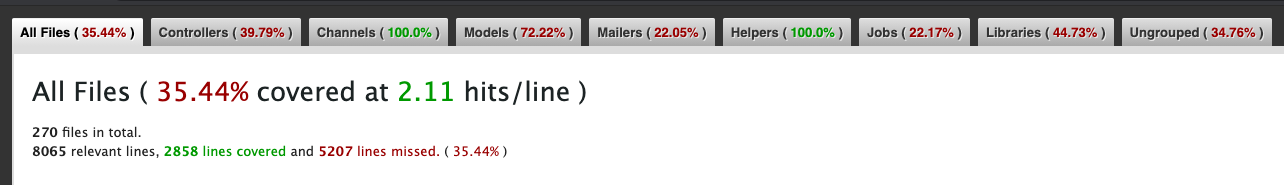
\includegraphics[width=\linewidth]{figures/testing/testing_original.png}
    \caption{Cobertura inicial del ERP (captura tomada el 3 de agosto de 2021).}
    \label{fig:testing_original}
  \end{figure}

  Dado que \textit{Hive}, en agosto, tenía aproximadamente 8000 líneas de código, el proceso del aumento de la cobertura del \textit{testing} comenzó mediante la revisión y mapeo de todos los archivos existentes y su estado de cobertura de pruebas. En otras palabras, se revisó todo el código fuente del ERP para saber cuáles archivos eran cubiertos por las pruebas automatizadas, cuáles no y cuáles requerían correcciones. De esta manera se podía ver con claridad en qué partes se tenía que enfocar los esfuerzos de trabajo y se podía saber cuáles archivos era más críticos de revisar y probar.

  El alumno realizó el mapeo de los archivos junto a Tomás Burotto y dejaron los registros en una sección especial de Jira. Esta documentación se organizó por secciones y subsecciones de archivos y carpetas, siguiendo la misma estructura de \textit{Hive}. Una vez que se transpasaron todos los archivos, se procedió a ponerles etiquetas del estado en que se encontraban, tal como se puede observar en la figura \ref{fig:mapeo_tests}.
  
  \begin{figure}
    \centering
    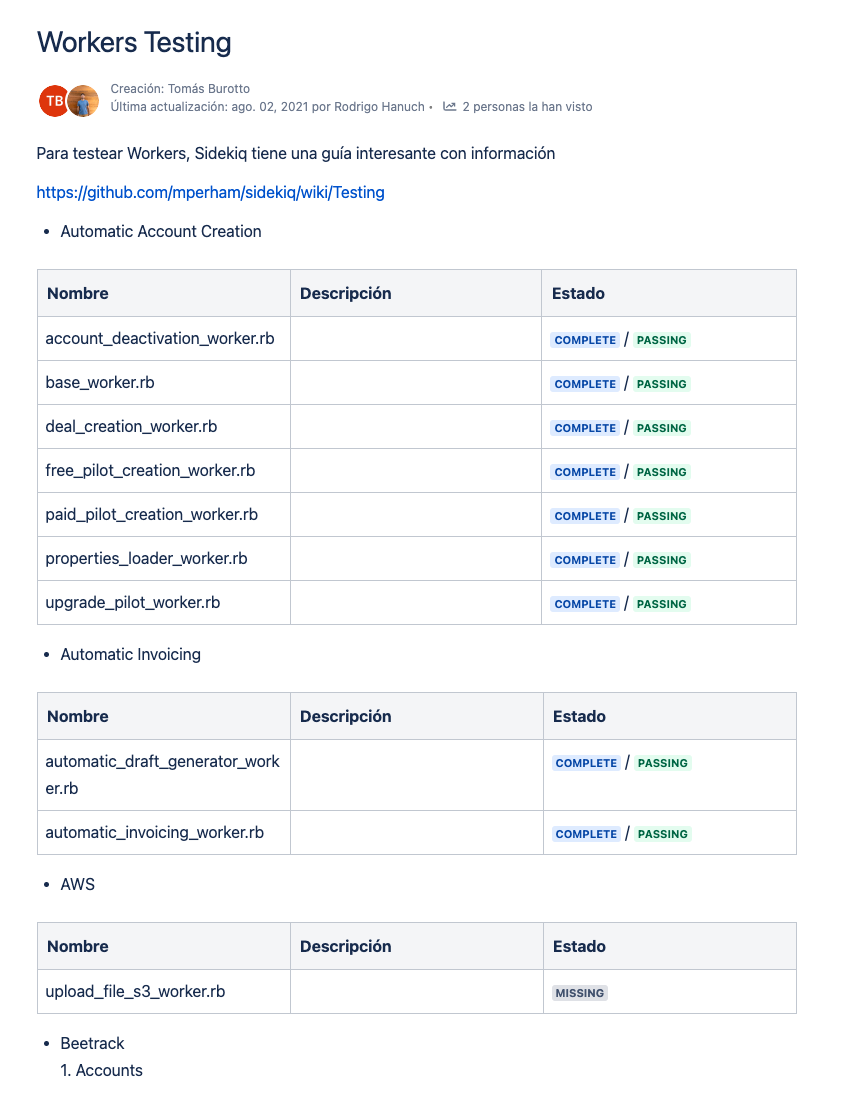
\includegraphics[width=0.75\linewidth]{figures/testing/mapeo_tests_existentes.png}
    \caption{Clasificación y etiquetado de los diferentes archvios y sus estados.}
    \label{fig:mapeo_tests}
  \end{figure}

  Se decidió tener 3 estados para la cobertura: ``\textit{complete}'', en el cual 100\% de las líneas correspondientes del archivo eran cubiertas, ``\textit{partial}'', para indicar que no todas las líneas del archivo eran cubiertas y ``\textit{none}'', para indicar que el archivo de pruebas existía, pero ninguna línea era cubierta. Por otro lado, también existían 3 etiquetas para el estado en que se econtraban las pruebas: ``\textit{passing}'' que aplicaba en caso de que todos los \textit{test} estuviesen pasando, ``\textit{failing}'' para indicar que una o más pruebas fallaban y ``\textit{skipped}'', que indicaba que una o más de las pruebas eran saltadas. Finalmente, se hizo una etiqueta adicional llamada ``\textit{missing}'' que se aplicó en el caso de que no existiese el archivo de pruebas correspondiente.
  
  Una vez que el alumno tuvo visibilidad del estado del \textit{testing} de la aplicación, este procedió a programar las pruebas automatizadas del código existente. Esto implicó el crear los archivos faltantes para el código que no era probado y leer el código existente, de manera de poder realizar pruebas adecuadas y no simplemente hacer pruebas que pasaran con cualquier resultado. La pricipal ventaja de realiazr pruebas muy detalladas es que permite tener un desgolse muy granular de qué falla en caso de que falle algo dentro del sistema, de manera de que se pueda corregir rápidamente y sin mayor conflicto. En particular, el alumno se enfocó en realizar pruebas automatizadas para la sección de \textit{workers}. El principal motivo del enfoque en estos archvios es debido a que los \textit{workers}, son procesos que corren de manera asíncrona del código principal del ERP y que son automatizaciones sensibles, como, por ejemplo, la generación de facturas y pre-facturas de manera automática, notificación a usuarios internos de la empresa, y cambios de estados en los contratos y datos de Hubspot, los cuales son vistos por los vendedores.

  Luego de que el estudiante cumpliera la meta establecida, este procedió a la siguiente tarea, la cual consistió en el cambió del \textit{deployment code} de Circle CI. El flujo de puesta en producción de Circle CI funciona mediante la declaración de pasos a seguir al momento de hacer un \textit{code deploy}. Previamente, la implementación de este código solamente contenía la compilación de los archivos y subida de estos a GKE. Para poder realizar la automatización de las pruebas en este entorno, se tuvo que levantar una imagen virtual de PostgreSQL en el contenedor de Circle CI y hacer que no finalizara su conexión luego de que se construyera, esto dado que para correr RSpec (el comando utilizado para correr las pruebas), se tiene que tener entradas en las bases de datos y para esto se tiene que tener una conexión abierta.

  El código que el alumno escribió para el flujo de Circle CI fue hecho de tal manera de que tuviese 2 pasos, en primer lugar las pruebas automatizadas, y luego, en caso de que el primer paso fuese existoso, el segundo paso fuese el \textit{deploy} y compilación del código para ser puesto en producción. Lo anterior permite que se pueda cortar el flujo en caso de que el primer paso falle, liberando antes los servidores que se utilizan de manera común en Beetrack para hacer \textit{deployment} tanto de los productos principales, como del \textit{software} interno de la emprsa. En la figura \ref{fig:flujo_circle_ci} se puede observar tanto el cambio de un flujo único sin pruebas automatizadas a uno con pruebas y el hecho de que cuando falla RSpec, el flujo se corta de inmediato, evitando el poner código defectuso en producción.

  \begin{figure}
    \centering
    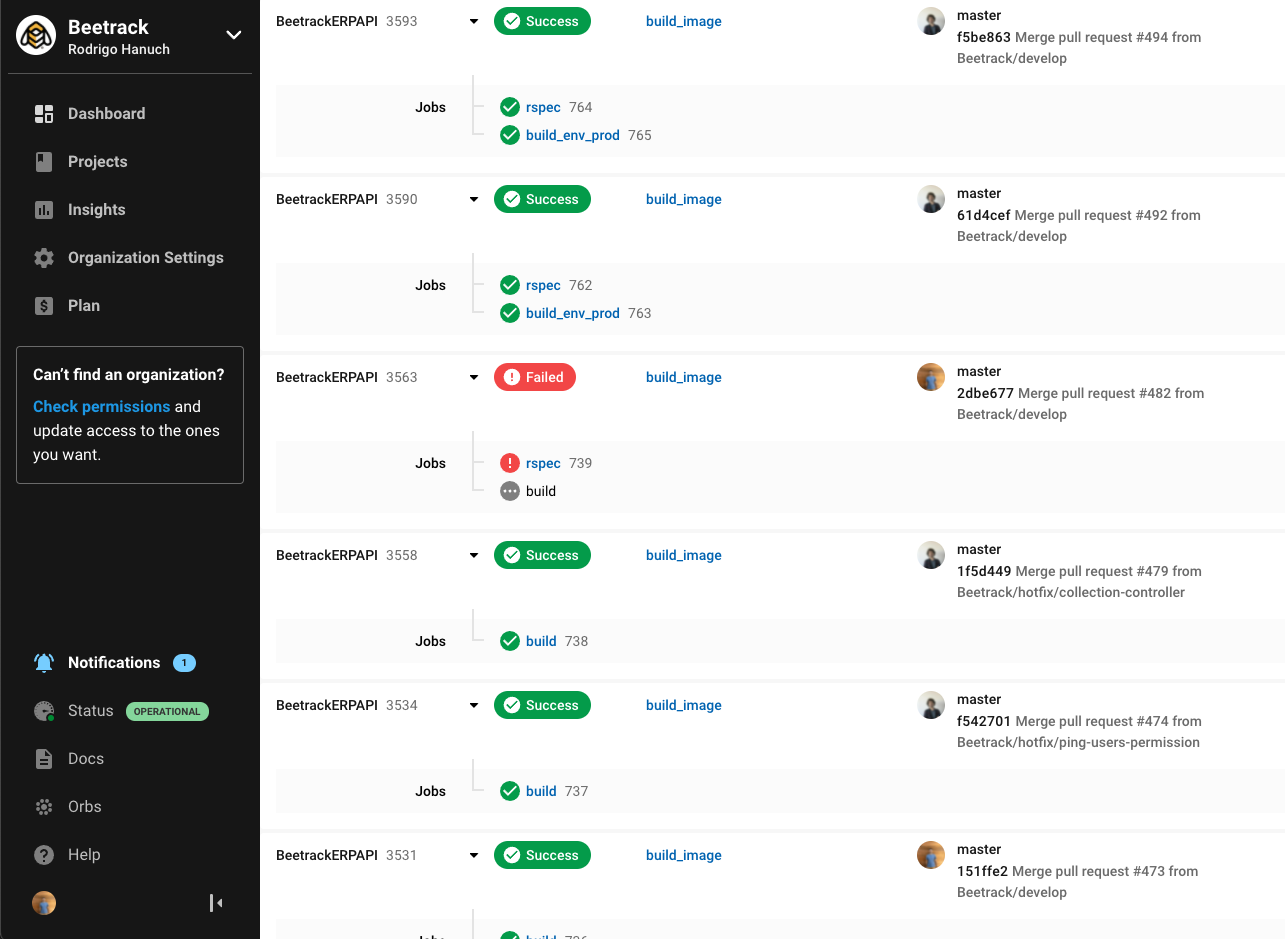
\includegraphics[width=\linewidth]{figures/testing/circle_ci_flow.png}
    \caption{Cambio en flujos de Circle CI y falla de \textit{RSpec} previa a la puesta en producción del código.}
    \label{fig:flujo_circle_ci}
  \end{figure}

\section{Resultados}

  Los principales resultados obtenidos de este proyecto fueron superiores a los propuestos originalmente. En particular se logó lo siguiente:
  
  \begin{enumerate}
    \item Cobertura de final de 64,04\% en \textit{Hive}.
    
    Se logró una cobertura de un 64,04\% del ERP, tal como se puede ver en la figura \ref{fig:testing_final}. Esto fue posible mediante la \textbf{simulación} de la ejecución de código previo a su puesta en producción y la aplicación de \textbf{conocimientos avanzados} de \textit{testing} para el \textit{framework} de RoR. Sumado a esto, también se tuvo extremo cuidado al momento de desarrollar las pruebas, evitando el escribir contraseñas o información sensible en estos mediante el uso de las herramientas proveídas por Rails, \textbf{cumpliendo con restricciones técnicas y éticas} para evitar que estas sean filtradas de manera pública a internet.
    
    \begin{figure}[H]
      \centering
      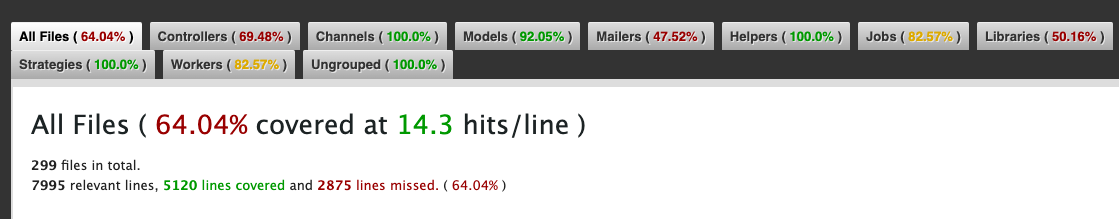
\includegraphics[width=\linewidth]{figures/testing/testing_final.png}
      \caption{Cobertura final del ERP (captura tomada el 15 de noviembre de 2021).}
      \label{fig:testing_final}
    \end{figure}

    \item Escritura de más de 2800 líneas de pruebas automatizadas.
    
    El incremento de la cobertura se logró mediante la escritura o modificación de 115 archivos con un total de 2816 líneas de código nuevas dedicadas exclusivamente a la automatización del proceso de pruebas, lo cual se puede ver en la figura \ref{fig:testing_file_commits}.

    \begin{figure}[H]
      \centering
      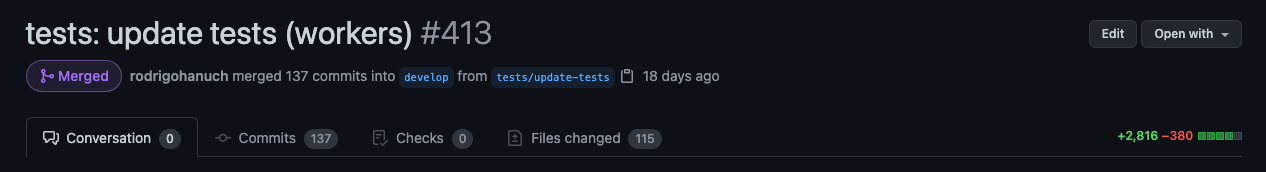
\includegraphics[width=\linewidth]{figures/testing/testing_file_commits.png}
      \caption{Archivos modificados y generados durante creación de nuevas pruebas.}
      \label{fig:testing_file_commits}
    \end{figure}

    \item Implementación de flujo de integración continua con pruebas automatizadas.
    
    La implementación del flujo de pruebas automatizadas en Circle CI tiene como principal resultado el incremento en confiabilidad del código escrito, y, por lo tanto, la disminución del \textit{downtime} generado por líneas no probadas para el equipo \textit{TechOps} y para la aplicación de \textit{Hive}. Sumado a lo anterior, esta implementación también consideró un flujo con menor cantidad de código al reescribir, en gran parte, los comandos que generaban los \textit{deployments} a GKE, reutilizando código y haciéndolo más legible al aplicar \textbf{patrones de diseño de \textit{software}} y eliminando muchos \textit{code smells} (antipatrones de diseño, que ocurren cuando el código no sigue estándares y que pueden indicar problemas más profundos \cite{code_smells}).

  \end{enumerate}
 